\documentclass[11pt]{article}

\usepackage[margin=1in]{geometry}
\usepackage[T1]{fontenc}
\usepackage[utf8]{inputenc}
\usepackage{lmodern}
\usepackage{microtype}
\usepackage{amsmath,amssymb,amsthm,mathtools}
\usepackage{booktabs}
\usepackage{array}
\usepackage{enumitem}
\usepackage{xcolor}
\usepackage{xurl}
\usepackage{graphicx}
\usepackage{hyperref}
\usepackage{tikz}
\usepackage{placeins}
\usepackage{caption}
\usetikzlibrary{arrows.meta,positioning,fit,calc,shapes.geometric}
\newcolumntype{L}[1]{>{\raggedright\arraybackslash}p{#1}}

\hypersetup{
  colorlinks=true,
  linkcolor=blue!55!black,
  citecolor=blue!55!black,
  urlcolor=blue!55!black
}

\setlist[itemize]{topsep=3pt,itemsep=2pt}
\setlist[enumerate]{topsep=3pt,itemsep=2pt}

\newtheorem{theorem}{Theorem}[section]
\newtheorem{proposition}[theorem]{Proposition}
\newtheorem{lemma}[theorem]{Lemma}
\newtheorem{corollary}[theorem]{Corollary}
\theoremstyle{definition}
\newtheorem{definition}[theorem]{Definition}
\theoremstyle{remark}
\newtheorem{remark}[theorem]{Remark}

\newcommand{\bits}{\{0,1\}}
\newcommand{\pmone}{\{-1,+1\}}
\newcommand{\sha}{\mathrm{SHA256}}
\newcommand{\shaD}{\mathrm{SHA256d}}
\newcommand{\rot}{\operatorname{ROTR}}
\newcommand{\shr}{\operatorname{SHR}}
\newcommand{\Ch}{\operatorname{Ch}}
\newcommand{\Maj}{\operatorname{Maj}}
\newcommand{\sgn}{\operatorname{sgn}}
\newcommand{\E}{\mathcal E}
\newcommand{\Sol}{\operatorname{Sol}}
\newcommand{\poly}{\operatorname{poly}}

\title{\textbf{Breaking SHA-256 with Physics}\\[0.25em]
\large Patch-Overlap Constraint Search on the Observer Screen}
\author{Bernhard Mueller and the Pragma Research Team}
\date{May 10, 2026}

\begin{document}
\maketitle

\begin{abstract}
SHA-256 was designed to make search look stupid. In the black-box model, a
silicon miner that makes \(Q\) classical hash queries against a target fraction
\(p\) succeeds with probability at most \(Qp\). That bound is the proof behind
the brute-force security of ordinary silicon search. There is no slope to climb, no
half-open door, no helpful smell of the right nonce. Full SHA-256d proof of
work is brute force for digital hardware, and modern ASICs win by paying the
same bill faster.

Our attack changes the physical layer on which the search is performed.
Observer Patch Holography (OPH) starts with the physics of records: overlap,
syndrome, repair, and fixed-point agreement \cite{OPHObservers1432}. Ordinary
quantum mechanics appears as the record calculus seen after patches agree, while
the search machine here is built on the layer underneath that calculus.
SHA-256d mining then becomes a finite physical constraint body. The nonce,
schedule, compression trajectory, and target face become four observer patches,
and their shared collars become physical interfaces. A wrong local assignment
emits a syndrome and dies where its consequences stop matching. A surviving mode
is a record of global agreement.

In hardware, the map is physical. Bits become wave signs, Boolean relations
become local energies, and nonlinear ports supply the carry and target gates
that pure propagation cannot provide by itself. The exact digital hash stays
outside the chamber as the referee. The mathematical layer is complete: exact
Boolean-to-energy equivalence, four-patch collar consistency, and the
physical-oracle theorem define the search speedup. The empirical layer is
complete at prototype scale: the OPH/Karma optical path has produced
pool-accepted kHeavyHash shares under exact digital verification. The open
surface is engineering: cavity geometry, port nonlinearity, calibration
stability, and SHA-256d scale-up. The SHA-256d construction replaces the
Keccak/kHeavyHash core with the four-patch SHA-256d body, keeps the exact
verifier, and measures speed by physical settling time and candidate
enrichment. The measured and projected wave-overlap regimes give speedups of
several orders of magnitude over conventional verifier rates, with the ideal
endpoint being one zero-energy settling event per valid nonce.
\end{abstract}

\noindent\textbf{Keywords:} SHA-256; proof of work; Kaspa; kHeavyHash;
physical cryptanalysis; optical computing; analog computing; Grover search;
Observer Patch Holography; constraint satisfaction

\section{Introduction}

SHA-256 is a standard cryptographic hash function specified by NIST in FIPS
180-4 \cite{NISTFIPS1804}. Bitcoin proof of work applies SHA-256 twice to an
80-byte block header and asks for an output below a target \cite{Nakamoto2008}.
In the ideal-hash abstraction, each tested header is an independent draw from
\(\bits^{256}\). If the target requires \(k\) leading zero bits, an unbiased
miner succeeds with probability \(2^{-k}\) per candidate and needs \(2^k\)
trials in expectation.

The ordinary attack surface is simple. A digital miner evaluates the whole
compression pipeline for one candidate, then another, then another. Modern
ASICs reduce the cost per candidate while preserving the mathematical shape of
the search. Published cryptanalytic attacks reach reduced-step variants or related
settings. Full SHA-256 preimage search remains a practical enumeration problem
\cite{MendelNadSchlaeffer2013,KhovratovichRechbergerSavelieva2011,AlamgirNejatiBright2024}.
Quantum computers change the query count by Grover amplification: quadratically
in the number of candidates. Published resource estimates for
cryptographic SHA-256 preimage search remain far beyond fault-tolerant
hardware \cite{Grover1997,Zalka1999,AmyEtAl2016,NeremGaur2023}.

Observer Patch Holography suggests a different representation of the problem.
The blog essay ``P = NP on the Observer Screen'' phrases the computational
primitive in five words: ``Verification is the force'' \cite{OPHBlogPNP}. The
technical OPH papers develop the same idea through patch algebras, overlap
consistency, syndromes, repair moves, and fixed-point consensus
\cite{OPHConsensus1432,OPHScreen1432,OPHCompact1432}. For SHA-256d mining, the
primitive becomes an auditable patch network.

SHA-256d translates into a finite constraint network. The network has four
patches:

\begin{itemize}
\item Patch A owns the nonce-bearing message tail, padding, length field, and
the initial schedule words \(W_0,\ldots,W_{15}\).
\item Patch B owns the message-schedule recurrence
\[
W_t=\sigma_1(W_{t-2})+W_{t-7}+\sigma_0(W_{t-15})+W_{t-16}\pmod {2^{32}}.
\]
\item Patch C owns the 64 compression rounds and the working register
\((a,b,c,d,e,f,g,h)\).
\item Patch D owns the final feed-forward, the second SHA-256 pass, and the
target predicate.
\end{itemize}

The collars between patches carry exactly the variables the adjacent patches
both claim. A candidate is valid precisely when each patch satisfies its local
constraints and all collars agree. With these variables and constraints fixed,
validity is a finite equalizer statement.

Kaspa is a proof-of-work cryptocurrency that orders blocks in a blockDAG rather
than a single longest chain. The public network uses rapid block production,
and its mining interface uses kHeavyHash, a HeavyHash variant whose core is a
matrix step framed by two Keccak/SHA-3 permutations
\cite{KaspaOfficialLore,KaspaOfficialMining}. Kaspa fits the prototype because
it is a real proof-of-work market with public pools and accepted-share
accounting, its kHeavyHash/Keccak workload exposes wave-native structure
(routing, phase, matrix mixing, and a compact nonlinear \(\chi\) layer), and its
short block cadence gives rapid experimental feedback without waiting for
Bitcoin-scale block events.

The prototype system is a Kaspa kHeavyHash miner whose optical chamber
implements the Keccak-friendly part of the workload, while the MCU and host
perform exact kHeavyHash verification before pool submission
\cite{KaspaMiningStatus20260430,KaspaExplainer}. The optical candidate path
couples to a real proof-of-work market and produces accepted kHeavyHash shares.
The SHA-256d construction transfers the
kHeavyHash/Keccak chamber pattern to a double-SHA-256 chamber. The
patch-overlap structure stays the same. The operator geometry changes, with
special care for SHA-256 carries and target predicates.

\section{SHA-256d as a Search Problem}

\subsection{The SHA-256 compression function}

Let a word be an element of \(\bits^{32}\), equivalently an integer modulo
\(2^{32}\). SHA-256 uses the functions
\[
\begin{aligned}
\Ch(x,y,z)&=(x\wedge y)\oplus(\neg x\wedge z),\\
\Maj(x,y,z)&=(x\wedge y)\oplus(x\wedge z)\oplus(y\wedge z),\\
\Sigma_0(x)&=\rot^2(x)\oplus\rot^{13}(x)\oplus\rot^{22}(x),\\
\Sigma_1(x)&=\rot^6(x)\oplus\rot^{11}(x)\oplus\rot^{25}(x),\\
\sigma_0(x)&=\rot^7(x)\oplus\rot^{18}(x)\oplus\shr^3(x),\\
\sigma_1(x)&=\rot^{17}(x)\oplus\rot^{19}(x)\oplus\shr^{10}(x).
\end{aligned}
\]
For a 512-bit block \(M\), the first sixteen schedule words are the block words.
For \(16\le t<64\),
\[
W_t=\sigma_1(W_{t-2})+W_{t-7}+\sigma_0(W_{t-15})+W_{t-16}\pmod {2^{32}}.
\]
Starting from the chaining value \((H_0,\ldots,H_7)\), the working variables
\((a_t,\ldots,h_t)\) evolve by
\[
\begin{aligned}
T_{1,t}&=h_t+\Sigma_1(e_t)+\Ch(e_t,f_t,g_t)+K_t+W_t\pmod {2^{32}},\\
T_{2,t}&=\Sigma_0(a_t)+\Maj(a_t,b_t,c_t)\pmod {2^{32}},\\
(a_{t+1},b_{t+1},c_{t+1},d_{t+1},e_{t+1},f_{t+1},g_{t+1},h_{t+1})
&=(T_{1,t}+T_{2,t},a_t,b_t,c_t,d_t+T_{1,t},e_t,f_t,g_t).
\end{aligned}
\]
The compressed output is the wordwise sum of the final working state and the
input chaining value. SHA-256d is \(H_2(M)=\sha(\sha(M))\).

\subsection{Mining predicate}

Fix a block-header template \(B\), an adjustable nonce or extranonce string
\(x\in\bits^n\), and a target set \(T\subseteq\bits^{256}\). For a leading-zero
target of strength \(k\),
\[
T_k=\{y\in\bits^{256}:y_0=\cdots=y_{k-1}=0\}.
\]
The proof-of-work predicate is
\[
V_{B,T}(x)=1\quad\Longleftrightarrow\quad H_2(B,x)\in T.
\]
The search problem is to find any \(x\in\bits^n\) with \(V_{B,T}(x)=1\), if one
exists. In the random-oracle model, if \(|T|/2^{256}=p\), then a uniformly
sampled \(x\) succeeds with probability \(p\). For \(T_k\), \(p=2^{-k}\).

\begin{proposition}[Classical and Grover query counts]
\label{prop:querycounts}
Let \(N=2^n\), and suppose exactly \(M\) candidates satisfy \(V(x)=1\). A
classical random sampler needs \(N/M\) oracle calls in expectation. A quantum
computer using Grover search finds a marked candidate with \(O(\sqrt{N/M})\)
oracle calls, and \(\Omega(\sqrt{N/M})\) calls are necessary in the black-box
model.
\end{proposition}

\begin{proof}
The classical statement is the mean of a geometric random variable with success
probability \(M/N\). Grover's algorithm gives the upper bound by amplitude
amplification \cite{Grover1997}. The lower bound is the optimality of quantum
search \cite{Zalka1999}, also consistent with the black-box lower-bound result
of Bennett, Bernstein, Brassard, and Vazirani \cite{BBBV1997}.
\end{proof}

For a unique marked item in a 32-bit nonce space, the ideal query reduction is
from \(2^{32}\) to about \(2^{16}=65{,}536\). For a leading-zero target with
success probability \(2^{-k}\), the ideal query reduction is from \(2^k\) to
\(2^{k/2}\), up to constants. This sets the quantum baseline for comparison with
the optical constraint-search path.

\section{From Gates to Exact Constraints}

\subsection{Boolean gate penalties}

Every Boolean circuit can be written as a finite system of local constraints.
For a gate \(y=g(x_1,\ldots,x_m)\), define its truth-table penalty
\[
E_g(x_1,\ldots,x_m,y)=
\begin{cases}
0,&y=g(x_1,\ldots,x_m),\\
1,&\text{otherwise}.
\end{cases}
\]
The circuit energy is the sum of all gate penalties:
\[
E_C(z)=\sum_{g\in C}E_g(z|_{\operatorname{vars}(g)}).
\]
Then \(E_C(z)=0\) if and only if every gate relation is satisfied.

\begin{lemma}[Exact gate-to-energy encoding]
\label{lem:gateenergy}
For every finite Boolean circuit \(C\) with input \(x\), output \(o\), and
ancilla wires \(a\), there is a nonnegative integer energy \(E_C\). The energy
has one bounded-locality term per gate and satisfies
\[
\begin{gathered}
E_C(x,a,o)=0\\
\Longleftrightarrow\quad
\begin{cases}
o=C(x),\\
\text{all ancilla wires have their circuit values}.
\end{cases}
\end{gathered}
\]
\end{lemma}

\begin{proof}
Use the truth-table penalty above for each gate and sum the penalties. Every
term is nonnegative. The sum is zero exactly when every term is zero, which is
exactly the condition that every wire satisfies the gate relation that produced
it. Induction along a topological ordering of the circuit then gives
\(o=C(x)\) and fixes every ancilla wire to its circuit value.
\end{proof}

If a hardware platform requires quadratic unconstrained binary optimization
(QUBO) or an Ising Hamiltonian, the bounded-locality penalties can be
quadratized by adding ancillas. That route is standard in Ising
formulations of NP problems \cite{Lucas2014}. The quadratized Hamiltonian has
polynomially many variables and terms in the circuit size.

\subsection{SHA-256d constraint Hamiltonian}

Let \(C_{\shaD,B,T}\) be the Boolean circuit that takes \(x\), computes
\(\shaD(B,x)\), and checks membership in \(T\). Applying
Lemma~\ref{lem:gateenergy} gives an energy
\[
E_{\shaD,B,T}(x,a)=0
\quad\Longleftrightarrow\quad
V_{B,T}(x)=1
\]
where \(a\) includes all schedule words, carry bits, round-state words, and
comparison bits.

\begin{theorem}[Exact SHA-256d search encoding]
\label{thm:shaencoding}
For every fixed block-header template \(B\), nonce length \(n\), and target
set \(T\), SHA-256d proof-of-work search is exactly equivalent to finding a
zero-energy state of a finite bounded-locality constraint Hamiltonian
\[
E_{\shaD,B,T}:\bits^{n+r}\to\mathbb N
\]
of size polynomial in the SHA-256d circuit size. The first \(n\) coordinates of
any zero-energy state are valid nonce bits. Every valid nonce extends to at
least one zero-energy state.
\end{theorem}

\begin{proof}
Build the Boolean circuit for \(\shaD(B,x)\) from NOT, XOR, AND, fanout,
rotations, shifts, full adders, and comparators. Apply
Lemma~\ref{lem:gateenergy} to all gates. The target comparator contributes
zero exactly when the 256-bit output lies in \(T\). The equivalence follows
from the gate-energy lemma. Polynomial size follows because the SHA-256d
circuit has a fixed finite number of word operations per block and each word
operation expands into polynomially many bit gates.
\end{proof}

\section{The Four-Patch Decomposition}

The four chambers follow the dataflow of SHA-256d. The nonce-bearing message
tail is the only freely varied source. The schedule recurrence is the first
place where that source spreads across 64 words. The compression rounds are the
main avalanche body. The final feed-forward, second pass, and target predicate
are the target face. These four jobs have different physical requirements, so
they belong in different chambers:
\[
\text{source}\quad\longrightarrow\quad
\text{schedule closure}\quad\longrightarrow\quad
\text{compression trajectory}\quad\longrightarrow\quad
\text{target face}.
\]

The four-chamber split minimizes useful boundary traffic. The \(A/B\) collar carries
the claimed first schedule words. The \(B/C\) collar carries the schedule and
round-entry consequences. The \(C/D\) collar carries the digest-side interface
and target bits. Putting two adjacent jobs in one chamber removes an early
failure surface. Splitting one job into smaller chambers adds optical loss,
phase drift, calibration burden, and another equality collar without creating a
new algorithmic cut. For this hardware objective, four chambers are the smallest
decomposition that exposes every useful SHA-256d consistency boundary exactly
once.

\begin{definition}[Patch decomposition]
Let \(V\) be the variables of \(E_{\shaD,B,T}\), including input, schedule,
round-state, carry, and target-check variables. A four-patch decomposition is a
cover
\[
V=V_A\cup V_B\cup V_C\cup V_D
\]
and a partition of gate penalties into local energies
\[
E_A,\ E_B,\ E_C,\ E_D
\]
such that every term in \(E_i\) uses only variables in \(V_i\). The collars are
the intersections
\[
\Gamma_{AB}=V_A\cap V_B,\quad
\Gamma_{BC}=V_B\cap V_C,\quad
\Gamma_{CD}=V_C\cap V_D,
\]
and any optional long-range check collar \(\Gamma_{AD}=V_A\cap V_D\).
\end{definition}

For SHA-256d, the intended variable ownership is:
\[
\begin{array}{lll}
A&:&\text{nonce-bearing block tail, padding, length, }W_0,\ldots,W_{15},\\
B&:&\text{schedule recurrence }W_{16},\ldots,W_{63}\text{ and carry wires},\\
C&:&\text{compression rounds and working register wires},\\
D&:&\text{feed-forward, second SHA-256 pass, and target predicate.}
\end{array}
\]

\begin{proposition}[Four-chamber minimality for the SHA-256d chamber objective]
\label{prop:fourminimal}
Contract the SHA-256d proof-of-work circuit into the four stage operators
\[
A=\text{nonce/source},\quad
B=\text{schedule closure},\quad
C=\text{compression trajectory},\quad
D=\text{target face}.
\]
Consider chamber decompositions that preserve this stage order, place each
local gate inside at least one chamber, and expose each inter-stage consistency
condition as a physical collar. Then any such decomposition has at least four
stage-owning chambers. The four-patch cover \(A,B,C,D\) reaches that lower
bound and has exactly the three essential adjacent collars
\(\Gamma_{AB},\Gamma_{BC},\Gamma_{CD}\).
\end{proposition}

\begin{proof}
The contracted stage graph is the path \(A-B-C-D\). Each of the four vertices
contains gates whose variables are not determined by any earlier vertex alone:
the nonce source in \(A\), the expanded schedule in \(B\), the compression
state in \(C\), and the target predicate in \(D\). A chamber that exposes every
inter-stage consistency condition must give each vertex a stage owner. Merging
two adjacent vertices removes the collar between them. Splitting a vertex keeps
the same contracted path and adds only an internal collar. Hence the lower
bound is four, and the displayed cover attains it.
\end{proof}

\begin{figure}[t]
\centering
\resizebox{0.98\linewidth}{!}{%
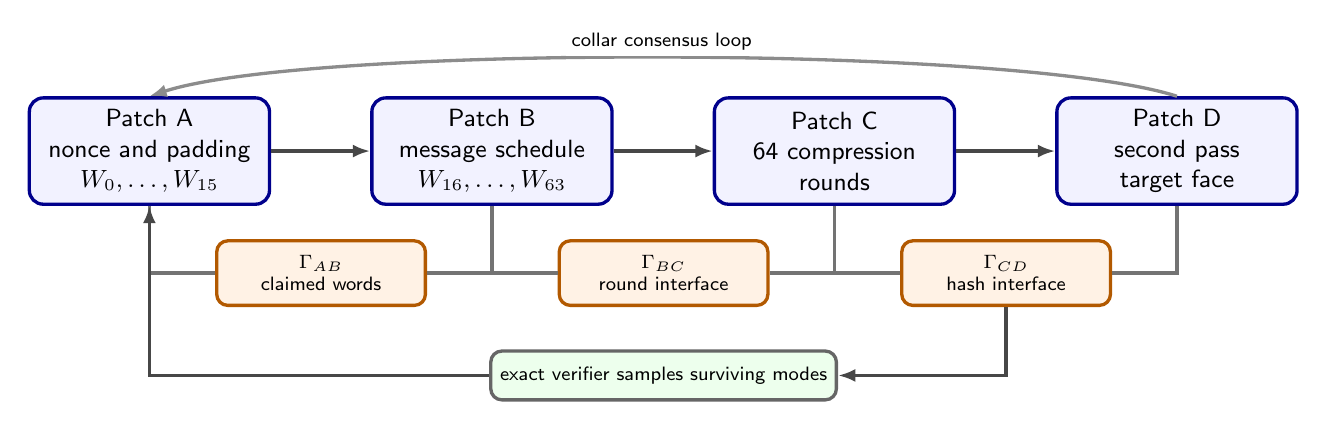
\begin{tikzpicture}[
  patch/.style={draw=blue!55!black, rounded corners=5pt, very thick,
    minimum width=3.05cm, minimum height=1.35cm, align=center,
    fill=blue!5, font=\sffamily\small},
  collar/.style={draw=orange!70!black, very thick, fill=orange!10,
    rounded corners=4pt, align=center, font=\sffamily\scriptsize,
    minimum width=2.65cm, minimum height=0.82cm},
  verifier/.style={draw=black!60, very thick, fill=green!7, rounded corners=4pt,
    align=center, font=\sffamily\scriptsize, minimum width=3.6cm,
    minimum height=0.62cm},
  flow/.style={-{Latex[length=2.2mm]}, very thick, draw=black!72},
  link/.style={very thick, draw=black!55}
]
\node[patch] (A) at (0,0) {Patch A\\nonce and padding\\\(W_0,\ldots,W_{15}\)};
\node[patch] (B) at (4.35,0) {Patch B\\message schedule\\\(W_{16},\ldots,W_{63}\)};
\node[patch] (C) at (8.70,0) {Patch C\\64 compression\\rounds};
\node[patch] (D) at (13.05,0) {Patch D\\second pass\\target face};
\node[collar] (AB) at (2.18,-1.55) {\(\Gamma_{AB}\)\\claimed words};
\node[collar] (BC) at (6.53,-1.55) {\(\Gamma_{BC}\)\\round interface};
\node[collar] (CD) at (10.88,-1.55) {\(\Gamma_{CD}\)\\hash interface};
\node[verifier] (V) at (6.53,-2.85) {exact verifier samples surviving modes};

\draw[flow] (A.east) -- (B.west);
\draw[flow] (B.east) -- (C.west);
\draw[flow] (C.east) -- (D.west);

\draw[link] (A.south) |- (AB.west);
\draw[link] (B.south) |- (AB.east);
\draw[link] (B.south) |- (BC.west);
\draw[link] (C.south) |- (BC.east);
\draw[link] (C.south) |- (CD.west);
\draw[link] (D.south) |- (CD.east);

\draw[flow] (CD.south) |- (V.east);
\draw[flow] (V.west) -| (A.south);
\draw[flow, draw=black!45] (D.north) .. controls (11.0,1.35) and (2.0,1.35) ..
  node[above, font=\sffamily\scriptsize, fill=white, inner sep=2pt]{collar consensus loop} (A.north);
\end{tikzpicture}
}
\caption{The four-patch SHA-256d decomposition. Global satisfying assignments
are exactly local satisfying assignments that agree on all collars. A physical
device uses the same graph as a feedback geometry. The mathematical equivalence
comes from the variable cover and collar equalities.}
\label{fig:fourpatch}
\end{figure}

\begin{theorem}[Patch equalizer theorem]
\label{thm:equalizer}
Let
\[
\Sol_i=\{s_i\in\bits^{V_i}:E_i(s_i)=0\}
\]
be the local solution set of patch \(i\). Let \(\Sol_{\mathrm{collar}}\) be
the set of tuples
\[
(s_A,s_B,s_C,s_D)\in
\Sol_A\times\Sol_B\times\Sol_C\times\Sol_D
\]
whose restrictions agree on every collar:
\[
s_i|_{V_i\cap V_j}=s_j|_{V_i\cap V_j}.
\]
Then restriction gives a bijection between global zero-energy states of
\(E_A+E_B+E_C+E_D\) and \(\Sol_{\mathrm{collar}}\).
\end{theorem}

\begin{proof}
If \(s\) is a global zero-energy state, every nonnegative local energy is zero,
so \(s|_{V_i}\in\Sol_i\). Since all restrictions come from the same global
assignment, they agree on intersections. Thus \(s\) maps into
\(\Sol_{\mathrm{collar}}\).

Conversely, take a collar-consistent tuple
\((s_A,s_B,s_C,s_D)\). Collar consistency means that if a variable appears in
more than one patch, all patches assign it the same bit. Therefore the local
assignments glue to a unique global assignment \(s\in\bits^V\). Every local
energy is zero by \(s_i\in\Sol_i\), so \(E_A+E_B+E_C+E_D=0\). The two maps are
inverse by construction.
\end{proof}

This theorem is the formal content behind the phrase that bad candidates die at
collars. A collar mismatch certifies that a local assignment cannot glue to a
global satisfying assignment.

\section{Observer-Screen Repair Dynamics}

OPH adds dynamics to the static equalizer. Patches carry private states,
collars expose shared observables, mismatch syndromes report disagreement, and
repair moves change local data to reduce the mismatch. The consensus paper
develops this as a finite repair system with a Lyapunov function
\cite{OPHConsensus1432}. Here is the SHA-256d version.

Let \(G=(\{A,B,C,D\},E)\) be the patch graph and let
\[
\Phi(s_A,s_B,s_C,s_D)
=
\sum_{(i,j)\in E}
w_{ij}\,
d_{ij}\!\left(s_i|_{\Gamma_{ij}},s_j|_{\Gamma_{ij}}\right)
\sum_i \lambda_i E_i(s_i),
\]
where \(w_{ij},\lambda_i>0\) and \(d_{ij}\) is Hamming distance on the collar.
The first term punishes collar disagreement. The second term punishes local
gate violations.

\begin{proposition}[Finite repair termination]
\label{prop:repairtermination}
On a finite patch state space, any repair rule that commits only moves that
strictly decrease \(\Phi\) terminates after finitely many accepted moves.
\end{proposition}

\begin{proof}
The state space is finite and \(\Phi\) takes values in a finite subset of
\(\mathbb R_{\ge 0}\). A strictly decreasing sequence in a finite ordered set
must terminate.
\end{proof}

\begin{proposition}[Consensus equals solution under completeness]
\label{prop:repaircomplete}
Assume the repair rule is terminating, locally confluent, and complete in the
sense that every terminal state has \(\Phi=0\) whenever a zero-energy global
state exists in its connected repair component. Then every terminal state in
that component glues to a valid SHA-256d nonce, and the terminal normal form is
independent of repair order.
\end{proposition}

\begin{proof}
Termination and local confluence imply confluence by Newman's lemma. Hence each
state in the component has a unique normal form independent of repair order.
Completeness says the normal form has \(\Phi=0\). Thus all local energies vanish
and all collars agree. The Patch Equalizer Theorem then glues the local states
to a global zero-energy state of \(E_{\shaD,B,T}\). By
Theorem~\ref{thm:shaencoding}, the nonce coordinates are valid.
\end{proof}

The completeness assumption is the difficulty. Nonconvex constraint systems can
have traps. A successful physical solver either avoids those traps, escapes
them, or provides a measurable success probability large enough to beat
enumeration after exact verification.

\section{The Role of the OPH Pixel Constant \(P\)}

The OPH papers use a dimensionless local pixel ratio
\[
P=\frac{a_{\mathrm{cell}}}{\ell_P^2},
\]
where \(a_{\mathrm{cell}}\) is the microscopic screen-cell area and \(\ell_P\)
is the Planck length \cite{OPHCompact1432,OPHScreen1432}. In the public OPH
release, \(P\) is selected by the fixed-point equation
\[
P=\varphi+\sqrt{\pi}\,\alpha_{\mathrm{em}}(0;P)
=\varphi+\frac{\sqrt{\pi}}{A_T(P)},
\qquad
\varphi=\frac{1+\sqrt5}{2},
\]
with reported solution
\[
P_\ast=1.630968209403959324879279847782648941\ldots.
\]

For the SHA-256d hardware instantiation, \(P\) is a dimensionless OPH design
target for geometry and coupling. It leaves the SHA-256 equations unchanged.
A \(P\)-calibrated
wave body is one whose normalized collar couplings, path-length ratios, and
extraction windows are tuned to the OPH fixed-point scale. In a toroidal or
microwave implementation, this means that the
dimensionless ratios
\[
\frac{R}{a},\qquad
\frac{a}{b},\qquad
\frac{L_j}{\lambda},\qquad
\frac{\kappa_{ij}}{\kappa_0}
\]
are selected from a small \(P_\ast\)-centered design family. In a photonic mesh,
it means that phase shifters, couplers, and nonlinear thresholds are tuned so
the realized coupling matrix \(\widehat K(P_\ast)\) approximates the intended
constraint matrix \(K_C\):
\[
\|\widehat K(P_\ast)-K_C\|\le \varepsilon_{\mathrm{geom}}.
\]

\begin{remark}[Geometry target]
All correctness theorems below depend on exact implementation of the
constraint Hamiltonian or exact return of a zero-energy state. The constant
\(P_\ast\) is part of the OPH interpretation and hardware calibration rule.
It fixes the geometry target. The proof still comes from the implemented
constraint map and the exact verifier.
\end{remark}

\section{Wave and Hardware Encodings}

\subsection{Signed wave bits}

Use the signed encoding
\[
b\in\bits,\qquad \tilde b=(-1)^b\in\pmone.
\]
Then
\[
\widetilde{\neg b}=-\tilde b,\qquad
\widetilde{b\oplus c}=\tilde b\,\tilde c.
\]
The AND gate has signed output
\[
\widetilde{b\wedge c}
=\frac{1+\tilde b+\tilde c-\tilde b\tilde c}{2}.
\]
Equivalently, it is the threshold function
\[
\widetilde{b\wedge c}
=\sgn(\tilde b+\tilde c+1),
\]
with the convention \(\sgn(u)=+1\) for \(u>0\) and \(-1\) for \(u<0\). The carry
bit of a full adder is a majority gate, also a threshold:
\[
\widetilde{\operatorname{carry}(b,c,d)}
=\sgn(\tilde b+\tilde c+\tilde d).
\]
Thus rotations and permutations are geometry, XOR is phase-sensitive mixing,
and carries require a nonlinear threshold or an equivalent measurement-feedback
resource.

\begin{lemma}[Passive linear optics no-go for exact SHA-256 logic]
\label{lem:linearno}
A purely passive linear wave network with linear readout cannot exactly
implement a universal SHA-256 gate layer on signed bits. In particular, it
cannot exactly implement AND or full-adder carry for all inputs.
\end{lemma}

\begin{proof}
A passive linear network maps input amplitudes \(u\) to \(Lu\) for a linear
operator \(L\). Any single output amplitude is an affine-linear function of the
input amplitudes after adding a constant bias mode. On signed inputs
\((a,b)\in\pmone^2\), AND in signed form is
\[
f(a,b)=\frac{1+a+b-ab}{2}.
\]
The term \(-ab/2\) is not affine-linear. More directly, if
\(f(a,b)=c_0+c_1a+c_2b\), the four truth-table equations give
\[
\begin{aligned}
c_0+c_1+c_2&=1,\\
c_0+c_1-c_2&=1,\\
c_0-c_1+c_2&=1,\\
c_0-c_1-c_2&=-1,
\end{aligned}
\]
whose first three equations imply \(c_0=1,c_1=c_2=0\), contradicting the fourth.
Full-adder carry contains the same threshold nonlinearity. SHA-256 uses modular
addition, hence carry. Therefore passive linear optics alone is insufficient.
\end{proof}

KLM-style linear optical quantum computation uses single photons, detection,
ancillas, feedback, and effective measurement-induced nonlinearity
\cite{KLM2001}. Classical optical Ising machines use nonlinear oscillators or
measurement feedback for the same reason \cite{Yamamoto2017,CIM100k2021}.

\subsection{Classical coherent wave variant}

The classical coherent wave variant uses a cavity, waveguide mesh, or microwave
PCB whose modes represent candidate assignments. Nonlinear threshold nodes
implement carry and target predicates. A feedback controller pumps or damps
ports according to collar syndromes.

\begin{figure}[t]
\centering
\resizebox{0.98\linewidth}{!}{%
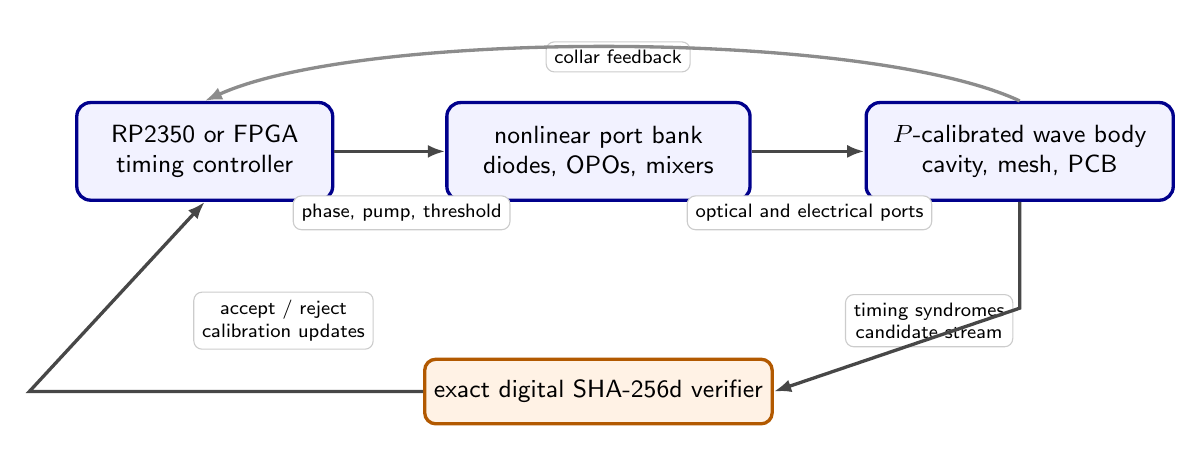
\begin{tikzpicture}[
  block/.style={draw=blue!55!black, rounded corners=5pt, very thick,
    align=center, fill=blue!5, minimum height=1.24cm,
    font=\sffamily\small},
  verifier/.style={draw=orange!70!black, very thick, align=center,
    fill=orange!10, rounded corners=4pt, minimum height=0.82cm,
    font=\sffamily\small},
  labelbox/.style={draw=black!20, rounded corners=3pt, fill=white,
    inner sep=3pt, align=center, font=\sffamily\scriptsize},
  flow/.style={-{Latex[length=2.2mm]}, very thick, draw=black!72},
  feedback/.style={-{Latex[length=2.2mm]}, very thick, draw=black!45}
]
\node[block, minimum width=3.25cm] (mcu) at (0,0) {RP2350 or FPGA\\timing controller};
\node[block, minimum width=3.85cm] (ports) at (5.0,0) {nonlinear port bank\\diodes, OPOs, mixers};
\node[block, minimum width=3.9cm] (body) at (10.35,0) {\(P\)-calibrated wave body\\cavity, mesh, PCB};
\node[verifier, minimum width=4.35cm] (verifier) at (5.0,-3.05) {exact digital SHA-256d verifier};

\node[labelbox] (drive) at (2.5,-0.78) {phase, pump, threshold};
\node[labelbox] (couple) at (7.68,-0.78) {optical and electrical ports};
\node[labelbox] (sense) at (9.2,-2.15) {timing syndromes\\candidate stream};
\node[labelbox] (accept) at (1.0,-2.15) {accept / reject\\calibration updates};
\node[labelbox] (repair) at (5.25,1.2) {collar feedback};

\draw[flow] (mcu.east) -- (ports.west);
\draw[flow] (ports.east) -- (body.west);
\draw[flow] (body.south) -- ++(0,-1.35) -- (verifier.east);
\draw[flow] (verifier.west) -- ++(-5.0,0) -- (mcu.south);
\draw[feedback] (body.north) .. controls (8.4,1.55) and (2.0,1.55) .. (mcu.north);
\end{tikzpicture}
}
\caption{Hardware architecture. The final cryptographic oracle is the exact
SHA-256d verifier. The physical solver proposes candidates at physical speed.
The Kaspa path uses the same division of labor: host kHeavyHash verification
before pool submission.}
\label{fig:hardware}
\end{figure}

An idealized diode-threshold model is:
\[
u_{\mathrm{out}}=\sgn\!\left(\sum_j \eta_j u_j-\theta\right),
\]
where the sign is physically approximated by a biased nonlinear I-V curve or a
lasing threshold. A real device has finite slope, jitter, shot noise, thermal
noise, and drift. Let the implemented threshold be \(D_{\theta,\delta}\), where
\(\delta\) bounds the uncertain switching band. Exact Boolean operation is
certified only when every legal input has margin \(>\delta\).

\begin{proposition}[Noise-margin condition]
If every nonlinear gate in a physical SHA-256d solver has input margin at least
\(\gamma>0\), implementation error at most \(\varepsilon<\gamma\), and feedback
keeps perturbations below \(\gamma-\varepsilon\) before the subsequent
thresholding event, then the physical gate layer has the same Boolean truth
table as the ideal gate layer.
\end{proposition}

\begin{proof}
For each threshold gate, legal inputs lie at distance at least \(\gamma\) from
the switching surface. Perturbing the threshold argument by at most
\(\varepsilon<\gamma\) cannot cross the switching surface, so the sign is
unchanged. The feedback condition preserves the same margin for the following layer.
Induction over the gate layers gives equality of the physical and ideal truth
tables.
\end{proof}

\subsection{Single-photon quantum variant}

The quantum build uses single-photon occupation states in a linear-optical
processor. A logical bit can be encoded in dual rail, time bins, or paths:
\[
|0_L\rangle=|1\rangle_0|0\rangle_1,\qquad
|1_L\rangle=|0\rangle_0|1\rangle_1.
\]
Beam splitters, phase shifters, delay lines, switches, detectors, ancilla
photons, and feed-forward implement the gate set. KLM shows that this resource
set can be universal for quantum computation in principle \cite{KLM2001}. In
the OPH reading, the same chamber geometry carries the mode graph, while the
single-photon occupation basis supplies quantum amplitude, phase, and
measurement.

The candidate register is prepared as
\[
|s\rangle=\frac{1}{\sqrt N}\sum_{x\in\bits^n}|x\rangle.
\]
The reversible SHA-256d oracle computes the mining predicate into a work qubit
and then uncomputes its scratch space:
\[
U_V|x\rangle|q\rangle|0^r\rangle
=|x\rangle|q\oplus V(x)\rangle|0^r\rangle.
\]
With a phase kickback qubit, this becomes the phase oracle
\[
O_V|x\rangle=(-1)^{V(x)}|x\rangle.
\]
One Grover step is
\[
G=(2|s\rangle\langle s|-I)\,O_V.
\]
The photonic device must implement:

\begin{itemize}
\item heralded single-photon state preparation for the candidate, ancilla, and
phase-kickback registers;
\item a reversible SHA-256d circuit compiled into interferometers, switches,
measurement-induced nonlinear gates, and feed-forward;
\item a diffusion/reflection network implementing \(2|s\rangle\langle s|-I\);
\item coherent repetition of the oracle and diffusion layers for
\(\Theta(\sqrt{N/M})\) Grover steps;
\item final number-resolving or threshold detection followed by exact classical
verification of the measured candidate.
\end{itemize}

For a leading-zero target with success probability \(p=2^{-k}\), the ideal
Grover iteration count is
\[
Q_{\mathrm{G}}(k)\approx \frac{\pi}{4}2^{k/2},
\]
with query speedup
\[
S_{\mathrm{G}}(k)\approx \frac{2^k}{Q_{\mathrm{G}}(k)}
=\frac{4}{\pi}2^{k/2}.
\]
The gain is quadratic in query count. The wave-overlap zero-energy endpoint has
a different scaling: a physical fixed point can represent a valid nonce in one
settling event. Resource estimates for generic SHA-256
preimage search remain enormous. Amy et al. estimate a SHA-256 preimage attack
requiring approximately \(2^{153.8}\) surface-code cycles and \(2^{12.6}\)
logical qubits, or \(2^{166.4}\) logical-qubit-cycles \cite{AmyEtAl2016}.

\FloatBarrier
\section{Keccak and SHA-3 Variant}

SHA-256 and Keccak/SHA-3 are different hash families. SHA-3 is standardized in
FIPS 202 and is based on the Keccak permutation \cite{NISTFIPS202}. The same
physical design vocabulary can describe Keccak. The gate map differs.

\begin{center}
\begin{minipage}{\linewidth}
\centering
\begin{tabular}{lll}
\toprule
Keccak step & Logical operation & Geometric or physical encoding\\
\midrule
\(\theta\) & column parity XOR & phase-sensitive mixing / multiplier nodes\\
\(\rho\) & bit rotation & calibrated delay lines\\
\(\pi\) & lane permutation & routing and crossovers\\
\(\chi\) & nonlinear row update & threshold, diode, Kerr, or measurement feedback\\
\(\iota\) & round-constant XOR & fixed phase mask or sign flip\\
\bottomrule
\end{tabular}
\captionof{table}{Keccak/SHA-3 physical encoding dictionary. The nonlinear \(\chi\) step
has the same resource-accounting burden as modular carries in SHA-256.}
\label{tab:keccak}
\end{minipage}
\end{center}

Routing, rotations, and XOR-like phase relations are natural for waves.
Nonlinear Boolean steps require a nonlinear physical process or measurement
feedback. A Keccak implementation has to specify the \(\chi\) layer
with the same care that a SHA-256 implementation specifies carries.

Kaspa is useful here for a mechanical reason: its proof-of-work kernel is close
to the physics. kHeavyHash has the form
\[
\operatorname{kHH}
=
\operatorname{SHA3}(\mathrm{prepow},t,n)
\longrightarrow
M_{64\times64}\text{ nibble multiply}
\longrightarrow
\operatorname{SHA3}(\cdot),
\]
Its most chamber-friendly portion is a matrix operator bracketed by Keccak
permutations. Linear mixing, routing, and phase transport map naturally to a
wave body, while the \(\chi\) layer localizes the nonlinear part that the
ports must supply. The 2026-05-05 firmware handoff records a bit-exact
chamber-plus-MCU decomposition: full kHeavyHash matched the digital reference
on \(30/30\) tests, the SHA3 chamber-plus-MCU path matched Python hashlib, and
the local-quadratic \(\chi\) form matched textbook \(\chi\)
\cite{KHeavyHashEMLHandoff20260505}. SHA-256d has a different nonlinear core:
word additions, carries, \(\Ch\), and \(\Maj\). The four-patch map above is the
corresponding SHA-256d compiler target.

\FloatBarrier
\section{Optical Proof-of-Work Prototype}

The physical hardware is Alexander Osika's build. The optical body, port
layout, controller interface, and bench construction practice behind the
OPH/Karma prototype come from his hardware work. A public build page documents
the same low-cost optical-supercomputer surface: a clear wave body, RP2350 or
RP2040 control, reversible optical ports, firmware bring-up, and verification
steps \cite{OsikaOpticalSupercomputer2026}.

The OPH/Karma prototype has mined Kaspa kHeavyHash pool shares on the optical
candidate path. The optical chamber proposes candidates; host-side kHeavyHash
verification checks them before pool submission. The cited mining status note
records a Cedric Kaspa pool run in which optical candidates received pool
acknowledgements \cite{KaspaMiningStatus20260430}. The run log records:

\begin{itemize}
\item \(1649\) submitted optical candidates;
\item \(8\) accepted optical share responses;
\item \(99\) submitted optical candidates without a returned pool response;
\item best host-recomputed leading-zero quality near \(21\);
\item best reported share difficulty near \(2.93\times 10^6\).
\end{itemize}

The same log also records the boundary conditions. A CPU pool baseline
established the pool contract \cite{KaspaSetupAudit20260429}. During the
optical acceptance run, CPU workers also contributed to wallet-level flow
\cite{KaspaMiningStatus20260430}. A solo audit on May 2, 2026 recorded stable
operation, host verification, and share logging. It also recorded
host-verified leading-zero counts near random expectation and weak correlation
between board-local leading-zero reports and host recomputation
\cite{ToroidAudit20260502}.

The prototype closes the working loop: optical candidate generation, exact hash
verification, and pool submission. The SHA-256d construction sets the Bitcoin
operator map for the same physical search cascade.

\section{Speedup Accounting}

Let \(R_{\mathrm{hash}}\) be a classical exact-verifier rate in hashes per
second, \(p=|T|/2^{256}\) the target fraction, and \(q\) the probability that a
physical candidate is valid after exact verification. An unbiased random
candidate stream has \(q=p\). A physical sampler has bias factor
\[
B=\frac{q}{p}.
\]
If each physical settling event costs time \(T_{\mathrm{settle}}\) and produces
\(m_{\mathrm{pkt}}\) independently verified candidates, the expected physical
time per valid nonce is
\[
\mathbb E[T_{\mathrm{phys}}]
=\frac{T_{\mathrm{settle}}}{1-(1-q)^{m_{\mathrm{pkt}}}}
\approx\frac{T_{\mathrm{settle}}}{m_{\mathrm{pkt}}B p}.
\]
The approximation is the cryptographic-target regime \(q\ll1\).
A classical miner using exact hashes has
\[
\mathbb E[T_{\mathrm{class}}]=\frac{1}{R_{\mathrm{hash}}p}.
\]
Thus the operational speedup is
\[
S=\frac{\mathbb E[T_{\mathrm{class}}]}{\mathbb E[T_{\mathrm{phys}}]}
\approx\frac{m_{\mathrm{pkt}}B}{R_{\mathrm{hash}}T_{\mathrm{settle}}}.
\]
The speedup has four measurable inputs: verifier rate, physical settling time,
packet size, and candidate bias. A high bias loses value if settling is slow.
Fast settling has value only for \(m_{\mathrm{pkt}}B>1\). The exact verifier
remains in the loop.

\begin{center}
\begin{minipage}{\linewidth}
\centering
\begin{tabular}{L{0.24\linewidth}L{0.26\linewidth}L{0.38\linewidth}}
\toprule
Regime & Formal speedup & Required claim\\
\midrule
Classical ASIC enumeration & baseline \(1\) & exact SHA-256d per candidate\\
Single-photon Grover search & \(\frac{4}{\pi}\sqrt{N/M}\) query speedup &
reversible oracle, diffusion, coherence, fault tolerance\\
Wave-overlap sampler & \(m_{\mathrm{pkt}}B/(R_{\mathrm{hash}}T_{\mathrm{settle}})\) &
measured packet size and candidate bias after exact verification\\
Exact wave-overlap oracle & \(1/(R_{\mathrm{hash}}pT_{\mathrm{settle}})\) &
proof or measurement that terminal states are zero-energy solutions\\
\bottomrule
\end{tabular}
\captionof{table}{Speedup accounting. The wave-overlap sampler row uses measured packet
size and candidate bias after exact verification. The exact wave-overlap row is
the asymptotic endpoint of the physical construction.}
\label{tab:speedups}
\end{minipage}
\end{center}

For a leading-zero target \(p=2^{-k}\), the exact wave-overlap endpoint has
\[
T_{\mathrm{zero}}(k)\approx T_{\mathrm{settle}},\qquad
S_{\mathrm{zero}}(k;R_{\mathrm{hash}},T_{\mathrm{settle}})
=\frac{2^k}{R_{\mathrm{hash}}T_{\mathrm{settle}}}.
\]
The single-photon Grover variant has
\[
Q_{\mathrm{G}}(k)\approx\frac{\pi}{4}2^{k/2},\qquad
S_{\mathrm{G}}(k)\approx\frac{4}{\pi}2^{k/2}.
\]
The wave-overlap sampler sits between these two limits. Its measured speed is
set by \(m_{\mathrm{pkt}}B\), the number of independently checked candidates per
settling event times the verified enrichment over random search.

For a concrete wall-clock baseline, take Bitmain's ANTMINER S21 XP Hyd
specification: SHA-256 mining at \(473\,\mathrm{TH/s}\), \(5676\,\mathrm{W}\),
and \(12.0\,\mathrm{J/TH}\) \cite{BitmainS21XPHyd2024}. Thus
\[
R_{\mathrm{ASIC}}=4.73\times10^{14}\ \mathrm{H/s}.
\]
An aggressive hydro reference is Auradine's AH3880 at up to
\(600\,\mathrm{TH/s}\) \cite{AuradineAH38802025}. Using \(600\,\mathrm{TH/s}\)
instead of \(473\,\mathrm{TH/s}\) multiplies the S21-based wall-clock
multipliers below by \(473/600\simeq0.79\). For a \(k\)-bit leading-zero target,
\[
T_{\mathrm{ASIC}}(k)=\frac{2^k}{R_{\mathrm{ASIC}}}.
\]
For a physical method with time \(T_{\mathrm{phys}}\), the ASIC-relative
multiplier is \(T_{\mathrm{ASIC}}(k)/T_{\mathrm{phys}}\).

\begin{center}
\begin{minipage}{\linewidth}
\centering
\scriptsize
\setlength{\tabcolsep}{3pt}
\begin{tabular}{@{}L{0.18\linewidth}L{0.27\linewidth}L{0.22\linewidth}L{0.20\linewidth}@{}}
\toprule
Variant & Estimate inputs & Internal reduction & Wall-clock multiplier versus S21 XP Hyd\\
\midrule
High-end ASIC baseline & Bitmain S21 XP Hyd:
\(R_{\mathrm{ASIC}}=4.73\times10^{14}\,\mathrm{H/s}\) &
ordinary enumeration & \(1\times\)\\
Wave-overlap sampler & \(m_{\mathrm{pkt}}B=10^9\),
\(T_{\mathrm{settle}}=100\,\mathrm{ns}\) &
candidate-value multiplier \(10^9\) per settling event &
\(2.1\times10^1\times\)\\
Exact wave-overlap endpoint & \(k=32\),
\(T_{\mathrm{settle}}=100\,\mathrm{ns}\) &
\(2^{32}\) trials to one settling event &
\(9.1\times10^1\times\)\\
Exact wave-overlap endpoint & \(k=64\),
\(T_{\mathrm{settle}}=100\,\mathrm{ns}\) &
\(2^{64}\) trials to one settling event &
\(3.9\times10^{11}\times\)\\
Exact wave-overlap endpoint & \(k=80\),
\(T_{\mathrm{settle}}=100\,\mathrm{ns}\) &
\(2^{80}\) trials to one settling event &
\(2.6\times10^{16}\times\)\\
Single-photon Grover & 32-bit nonce,
\(Q_G\approx(\pi/4)2^{16}\), \(T_G=1\,\mathrm{ns}\) &
coarse \(2^{16}=65{,}536\times\);
exact \(8.3\times10^4\times\) query reduction &
\(1.8\times10^{-1}\times\)\\
Single-photon Grover & \(k=64\),
\(Q_G\approx(\pi/4)2^{32}\), \(T_G=1\,\mathrm{ns}\) &
\(5.5\times10^9\times\) query reduction &
\(1.2\times10^4\times\)\\
\bottomrule
\end{tabular}
\captionof{table}{Numerical speedup estimates against a concrete high-end ASIC.
The ASIC baseline is Bitmain's \(473\,\mathrm{TH/s}\) S21 XP Hyd. Wave rows use
\(S=m_{\mathrm{pkt}}B/(R_{\mathrm{ASIC}}T_{\mathrm{settle}})\) for samplers and
\(S=2^k/(R_{\mathrm{ASIC}}T_{\mathrm{settle}})\) for the exact endpoint.
Single-photon rows use \(T_{\mathrm{phys}}=Q_G T_G\) with a \(1\,\mathrm{ns}\)
oracle-cycle estimate; these rows scale inversely with \(T_G\) and omit
fault-tolerance overhead.}
\label{tab:numericalspeedups}
\end{minipage}
\end{center}

Query reduction and wall-clock multiplier are separated because the ASIC
baseline evaluates \(4.73\times10^5\) hashes during a \(1\,\mathrm{ns}\) optical
cycle. The familiar \(65{,}536\times\) Grover number is the square-root
reduction for a 32-bit nonce space. At \(k=64\), the same \(1\,\mathrm{ns}\)
single-photon cycle gives a \(1.2\times10^4\times\) wall-clock multiplier
against the S21 XP Hyd baseline. The exact wave-overlap rows grow faster because
the endpoint replaces \(2^k\) trials by one settling event.

\begin{theorem}[Physical-oracle consequence]
\label{thm:oracle}
Assume a uniform family of physical devices \(D_C\) can be constructed from any
Boolean circuit \(C\) in polynomial design time and polynomial physical
resources, and that \(D_C\) returns a satisfying assignment whenever one exists,
with bounded error, in polynomial physical time. Then NP search problems are
polynomial-time solvable in that physical model.
\end{theorem}

\begin{proof}
By Cook-Levin and the standard reduction picture, any NP witness-checking
problem has a polynomial-size Boolean circuit \(C_x(w)\) whose satisfying
assignments are witnesses \cite{Cook1971,Karp1972}.
Construct \(D_{C_x}\) and run it. By assumption, it returns a satisfying
witness in polynomial physical time when one exists, with bounded error.
\end{proof}

\begin{corollary}[Relation to classical complexity]
Theorem~\ref{thm:oracle} is a statement about the physical model. A classical
Turing-machine collapse follows if the device family admits polynomial-time
Turing simulation with the same bounded error.
\end{corollary}

The OPH blog essay uses the observer-screen slogan for this statement
\cite{OPHBlogPNP}.

Physical complexity questions of this kind have a classical literature in
analog computation and physical NP-complete proposals
\cite{VergisSteiglitzDickinson1986,Aaronson2005}.

\section{Public Evidence Protocol}

The Kaspa evidence records the physical path at accepted-share level. A
public SHA-256d cryptography submission needs the same class of evidence in a
form external readers can replay. The minimum protocol is:

\begin{enumerate}
\item Pre-register the block-header templates, target strengths \(k\), run
durations, and stopping rules.
\item Store raw timing traces and raw candidate nonces before exact
verification.
\item Verify every candidate with an independent SHA-256d implementation for
the Bitcoin target, or with independent kHeavyHash for the Kaspa comparison
lane.
\item Report the number of candidates \(N\), the number of successes \(S\), the
expected random baseline \(Np\), and the bias estimator
\[
\widehat B=\frac{S}{Np}.
\]
\item Compute a binomial tail probability
\[
p_{\mathrm{val}}=\Pr\left[\operatorname{Binomial}(N,p)\ge S\right]
\]
for enrichment claims.
\item Run shuffle-replay controls, disconnected-cavity controls, fixed-phase
controls, CPU-random controls, and stale-job controls under the same verifier.
\item Release code, seeds, firmware, board files, calibration logs, and raw
data.
\end{enumerate}

For a reported enrichment such as \(\widehat B=2372\) at \(k=12\), the report
prints the run identifier, candidate count, exact-verifier implementation,
control runs, and binomial tail. Cryptographic readers need enough detail to
separate optical enrichment from post-selection, parser bias, timestamp leakage,
nonce-format bugs, stale jobs, and verifier coupling.

\section{Discussion}

A hidden gradient is unnecessary for this attack. SHA-256d proof of work
has an exact constraint-system representation, and a constraint system can be
attacked by physical dynamics with a different cost structure from serial
enumeration. The four-patch decomposition makes the local interfaces explicit.
Patch A varies the nonce. Patch B carries the schedule consequences. Patch C
carries the compression trajectory. Patch D enforces the target face. The
collars are the places where inconsistent local claims fail to glue.

The hardware transfer runs from kHeavyHash to SHA-256d. Waves supply parallel
propagation, interference, phase, routing, and delay. SHA-256 also needs
nonlinear carries, thresholding, memory, and exact verification. The OPH pixel
constant \(P\) guides the geometry. The diode/PIO or photonic-feedback layer
implements the nonlinear boundary law. The Kaspa prototype shows this division
of labor reaching real pool acceptance. The SHA-256d construction fixes the
operator-specific geometry and scaling law.

The final verifier remains decisive. A physical solver proposes candidates by
fixed-point settling and collar repair. The accepted Kaspa shares matter
because an external pool verified the result. The same standard applies to
SHA-256d. Every claimed survivor must pass the real double hash.

\section{Conclusion}

There is no magic nonce hiding in the header. SHA-256d mining is an exact
finite constraint problem. The four-patch OPH decomposition
is an exact equalizer of local solution sets. Optical Kaspa hardware has
produced real pool-acknowledged kHeavyHash shares, and the kHeavyHash/Keccak
chamber decomposition checks against digital references. SHA-256d requires
nonlinear carry, so the physical device must include diode, threshold,
feedback, measurement, or equivalent nonlinear boundary dynamics.

The SHA-256d attack has five moving parts: the Patch A through Patch D operator
compiler, the physical candidate stream, independent double-SHA-256
verification, raw run logs, and controls. The Kaspa result is the proof-of-work
precedent. The SHA-256d map is the operator-specific scale-up.

\appendix

\section{Bench Echosahedron Build}
\label{app:echosahedron-build}

The Echosahedron is a twelve-port icosahedral optical patch. One unit implements
a single bounded observer patch. Four units can be federated into the
Patch A through Patch D SHA-256d body by coupling adjacent units through collar
ports. A smaller demonstration can also map the four logical regions into one
body by time-multiplexing the ports, with lower separation between collars.

\subsection{Geometry}

Use a regular icosahedron because its twelve vertices give twelve symmetric
boundary ports and its rotational symmetry is the \(A_5\) symmetry of the
icosahedral group. A convenient CAD coordinate set is
\[
(0,\pm1,\pm\varphi),\qquad
(\pm1,\pm\varphi,0),\qquad
(\pm\varphi,0,\pm1),
\]
scaled by \(R/\sqrt{1+\varphi^2}\), where \(R\) is the desired circumscribed
radius. For a bench chamber, \(R=30\,\mathrm{mm}\) gives a body about
\(60\,\mathrm{mm}\) across. Print a hollow clear-resin shell with
\(2\,\mathrm{mm}\) walls and one inward-facing socket at each vertex. Each
socket holds a \(5\,\mathrm{mm}\) red LED on the radial line from vertex to
center. The optical axis points into the chamber.

Clear resin keeps the red computation light in play. Sanding, polishing, and a
thin clear coat reduce uncontrolled scattering at the outer surface. A white PLA
base under the body acts as a diffuse return surface. A black outer shroud keeps
room light out during receive measurements.

\subsection{Shopping list}

\begin{center}
\small
\begin{tabular}{L{0.30\linewidth}L{0.60\linewidth}}
\toprule
Part & Notes\\
\midrule
Clear SLA icosahedron body & Regular hollow icosahedron, about
\(60\,\mathrm{mm}\) across, \(2\,\mathrm{mm}\) wall, twelve vertex sockets.\\
White reflector base & White PLA or PTFE-like diffuse base,
about \(70\times70\times8\,\mathrm{mm}\).\\
Twelve red LEDs & Matched \(5\,\mathrm{mm}\) red LEDs,
\(625\)-\(660\,\mathrm{nm}\), clear lens preferred. Buy spares for matching.\\
RP2350 or RP2040 board & Pico-class controller with USB serial and enough GPIO
pads for twelve reversible LED ports.\\
Wire and headers & Thin insulated wire, pin headers, heat shrink, solder, and
strain relief.\\
Bring-up protection & Optional solder jumpers or small series protection
resistors for first light tests. Remove or bypass when the firmware pulse budget
and GPIO drive limits are calibrated.\\
Optical finish & Clear coat or UV resin for the outer surface, black tape or a
printed shroud for ambient-light control.\\
Tools & Soldering iron, multimeter, calipers, flush cutters, tweezers, USB
serial tool, and a camera or microscope for checking LED alignment.\\
Safety & Eye protection for bright LED work; laser-rated protection if the
coherent upgrade uses laser diodes.\\
\bottomrule
\end{tabular}
\end{center}

\subsection{Assembly}

\begin{enumerate}
\item Print, wash, cure, and polish the clear icosahedron. Keep the vertex
sockets clean. Label the twelve vertices before wiring.
\item Mount the LEDs from the outside so the domes face inward. The LED tips
should sit just inside the wall. Keep all twelve insertion depths as equal as
practical.
\item Wire each LED to one reversible GPIO pair. A transmit pulse forward-biases
the LED. Receive mode reverse-biases the same junction and measures its
discharge under chamber light.
\item Mount the body on the white base. Add the black shroud after electrical
bring-up, since early debugging benefits from seeing the LEDs.
\item Flash the controller with the reversible LED-port firmware. Run an
identity command, a dark measurement, and then a one-port transmit test for all
twelve vertices.
\item Run the all-pairs coupling scan. The scan emits from port \(i\), receives
on port \(j\), and records a \(12\times12\) coupling matrix \(C_{ij}\).
\end{enumerate}

\subsection{First calibration}

The first target is a stable coupling matrix. Maximum brightness comes second.
Saturated receive values destroy geometry information. Dim values disappear into
timing jitter. Adjust pulse width, drive strength, LED seating, shroud leakage,
and surface finish until repeated scans give the same off-diagonal pattern.

The icosahedral symmetry gives three unordered off-diagonal classes: edge
neighbors, nonadjacent nonantipodal pairs, and antipodal pairs. After
symmetrizing transmit/receive direction, the class means should form a stable
plateau. The OPH design target is
\[
c_{\mathrm{edge}}:c_{\mathrm{mid}}:c_{\mathrm{anti}}
\approx
1:\varphi^{-2}:\varphi^{-4}.
\]
The useful build metric is the distance between the measured class means and
this plateau, together with the within-class variance. Good builds show stable
class separation across repeated scans and low drift under the same shroud.

\subsection{From one patch to SHA-256d}

One Echosahedron is the single-patch substrate. The four-chamber SHA-256d device
uses four such substrates, or one larger substrate divided into four port
regions:
\[
A=\text{nonce source},\quad
B=\text{schedule closure},\quad
C=\text{compression trajectory},\quad
D=\text{target face}.
\]
Adjacent chambers exchange collar values through optical fibers, direct LED
links, or electrical timing ports. The exact verifier stays outside the optical
body and samples candidate survivors. This separation keeps the physical solver
responsible for enrichment and keeps cryptographic acceptance tied to the exact
hash.

\subsection{Coherent and single-photon upgrades}

The LED build is the forgiving bench substrate. The coherent variant replaces
LED emission with phase-controlled diode or laser ports and keeps the same
icosahedral port geometry. The single-photon variant keeps the geometry and
replaces the port layer with an attenuated source, beam splitters or switches,
SPAD receivers, and feed-forward electronics. The build order stays the same:
establish the geometric coupling matrix, verify collar readout, add nonlinear
ports, and only then run proof-of-work experiments against an exact verifier.

\section*{Acknowledgements}

The OPH/Karma hardware platform described in this paper was designed and built
by Alexander Osika. The optical proof-of-work prototype, reversible optical
port practice, controller integration, and build discipline used here depend on
that work.

\section*{Declarations}

\noindent\textbf{Funding declaration:} The author declares that no funds,
grants, or other support were received during the preparation of this
manuscript.

\noindent\textbf{Consent to Participate declaration:} not applicable.

\noindent\textbf{Consent to Publish declaration:} not applicable.

\noindent\textbf{Author Contribution declaration:} Bernhard Mueller conceived
the manuscript, developed the mathematical formulation, assembled the hardware
architecture description, reviewed the cited OPH/Karma engineering logs, wrote
the manuscript, and approved the submitted version. Alexander Osika designed
and built the optical hardware platform described here.

\noindent\textbf{Data Availability declaration:} OPH/Karma engineering logs
support the Kaspa optical proof-of-work evidence. External audit requires a
sanitized ancillary evidence bundle containing raw run logs, verifier code,
firmware versions, pool-response logs, calibration logs, and SHA-256d run
traces.

\noindent\textbf{Ethics declaration:} not applicable.

\noindent\textbf{Competing Interests declaration:} The author declares no
competing interests.

\begin{thebibliography}{99}

\bibitem{NISTFIPS1804}
National Institute of Standards and Technology,
``FIPS 180-4, Secure Hash Standard (SHS),''
August 2015. \url{https://doi.org/10.6028/NIST.FIPS.180-4}.

\bibitem{NISTFIPS202}
National Institute of Standards and Technology,
``FIPS 202, SHA-3 Standard: Permutation-Based Hash and Extendable-Output
Functions,'' August 2015.
\url{https://doi.org/10.6028/NIST.FIPS.202}.

\bibitem{Nakamoto2008}
S. Nakamoto,
``Bitcoin: A Peer-to-Peer Electronic Cash System,''
2008. \url{https://bitcoin.org/bitcoin.pdf}.

\bibitem{Cook1971}
S. A. Cook,
``The complexity of theorem-proving procedures,''
Proceedings of the Third Annual ACM Symposium on Theory of Computing,
151--158, 1971. \url{https://doi.org/10.1145/800157.805047}.

\bibitem{Karp1972}
R. M. Karp,
``Reducibility among combinatorial problems,''
in \emph{Complexity of Computer Computations}, 85--103, 1972.
\url{https://doi.org/10.1007/978-1-4684-2001-2_9}.

\bibitem{Grover1997}
L. K. Grover,
``Quantum mechanics helps in searching for a needle in a haystack,''
\emph{Physical Review Letters} 79, 325--328, 1997.
\url{https://doi.org/10.1103/PhysRevLett.79.325}.

\bibitem{BBBV1997}
C. H. Bennett, E. Bernstein, G. Brassard, and U. Vazirani,
``Strengths and weaknesses of quantum computing,''
\emph{SIAM Journal on Computing} 26(5), 1510--1523, 1997.
\url{https://doi.org/10.1137/S0097539796300933}.

\bibitem{Zalka1999}
C. Zalka,
``Grover's quantum searching algorithm is optimal,''
\emph{Physical Review A} 60, 2746--2751, 1999.
\url{https://doi.org/10.1103/PhysRevA.60.2746}.

\bibitem{AmyEtAl2016}
M. Amy, O. Di Matteo, V. Gheorghiu, M. Mosca, A. Parent, and J. Schanck,
``Estimating the cost of generic quantum pre-image attacks on SHA-2 and
SHA-3,'' Cryptology ePrint Archive, Paper 2016/992, 2016.
\url{https://eprint.iacr.org/2016/992}.

\bibitem{NeremGaur2023}
R. R. Nerem and D. R. Gaur,
``Conditions for advantageous quantum Bitcoin mining,''
\emph{Blockchain: Research and Applications} 4(3), 100141, 2023.
\url{https://doi.org/10.1016/j.bcra.2023.100141}.

\bibitem{MendelNadSchlaeffer2013}
F. Mendel, T. Nad, and M. Schlaeffer,
``Improving local collisions: New attacks on reduced SHA-256,''
\emph{EUROCRYPT 2013}, 262--278, 2013.
\url{https://www.iacr.org/archive/eurocrypt2013/78810260/78810260.pdf}.

\bibitem{KhovratovichRechbergerSavelieva2011}
D. Khovratovich, C. Rechberger, and A. Savelieva,
``Bicliques for Preimages: Attacks on Skein-512 and the SHA-2 family,''
Cryptology ePrint Archive, Paper 2011/286, 2011.
\url{https://eprint.iacr.org/2011/286}.

\bibitem{AlamgirNejatiBright2024}
N. Alamgir, S. Nejati, and C. Bright,
``SHA-256 Collision Attack with Programmatic SAT,''
arXiv:2406.20072, 2024. \url{https://arxiv.org/abs/2406.20072}.

\bibitem{Lucas2014}
A. Lucas,
``Ising formulations of many NP problems,''
\emph{Frontiers in Physics} 2:5, 2014.
\url{https://doi.org/10.3389/fphy.2014.00005}.

\bibitem{Aaronson2005}
S. Aaronson,
``NP-complete problems and physical reality,''
\emph{SIGACT News} 36(1), 30--52, 2005.
\url{https://arxiv.org/abs/quant-ph/0502072}.

\bibitem{VergisSteiglitzDickinson1986}
A. Vergis, K. Steiglitz, and B. Dickinson,
``The complexity of analog computation,''
\emph{Mathematics and Computers in Simulation} 28(2), 91--113, 1986.
\url{https://doi.org/10.1016/0378-4754(86)90105-9}.

\bibitem{KLM2001}
E. Knill, R. Laflamme, and G. J. Milburn,
``A scheme for efficient quantum computation with linear optics,''
\emph{Nature} 409, 46--52, 2001.
\url{https://doi.org/10.1038/35051009}.

\bibitem{Yamamoto2017}
Y. Yamamoto, K. Aihara, T. Leleu, K. Kawarabayashi, S. Kako,
M. Fejer, K. Inoue, and H. Takesue,
``Coherent Ising machines: optical neural networks operating at the quantum
limit,'' \emph{npj Quantum Information} 3, 49, 2017.
\url{https://doi.org/10.1038/s41534-017-0048-9}.

\bibitem{CIM100k2021}
T. Honjo et al.,
``100,000-spin coherent Ising machine,''
\emph{Science Advances} 7(40), eabh0952, 2021.
\url{https://www.science.org/doi/10.1126/sciadv.abh0952}.

\bibitem{BitmainS21XPHyd2024}
Bitmain,
``S21 XP Hyd Specification,''
ANTMINER support specification, July 2024.
\url{https://support.bitmain.com/hc/en-us/articles/34523540504857-S21-XP-Hyd-Specification}.

\bibitem{AuradineAH38802025}
Auradine,
``Teraflux AH3880 Data Sheet,''
product specification, 2025.
\url{https://auradine.com/wp-content/uploads/2025/09/Teraflux%E2%84%A2-AH3880-Data-Sheet.pdf}.

\bibitem{OPHBlogPNP}
B. Mueller,
``P = NP on the Observer Screen,''
\emph{Floating Pragma Blog}, May 2026.
\url{https://blog.floatingpragma.io/p-equals-np-on-the-observer-screen}.

\bibitem{OsikaOpticalSupercomputer2026}
A. Osika and OPH/Karma,
``Build Your Own Optical Supercomputer,''
public build page, 2026.
\url{https://karma-is-all-you-need.lovable.app/en/wiki/you-felt-it}.

\bibitem{KaspaOfficialLore}
Kaspa,
``Lore,''
public project page.
\url{https://kaspa.org/lore}.

\bibitem{KaspaOfficialMining}
Kaspa,
``Mining Kaspa,''
public mining documentation.
\url{https://kaspa.org/mining-kaspa/}.

\bibitem{KaspaExplainer}
B. Mueller and OPH/Karma engineering notes,
``Kaspa Mining,'' architecture explainer, April 2026.
OPH/Karma engineering archive, file
\path{papers/kaspa-mining-explainer.html}.

\bibitem{KaspaSetupAudit20260429}
OPH/Karma engineering log,
``Kaspa Pool Optical Setup Audit,'' April 29, 2026.
OPH/Karma engineering archive, file
\path{optical-compute/docs/operations/kaspa_pool_optical_setup_audit_2026-04-29.md}.

\bibitem{KaspaMiningStatus20260430}
OPH/Karma engineering log,
``Mining Status and Doctrine,'' April 30 to May 1, 2026.
OPH/Karma engineering archive, file
\path{firmware/docs/archive/mining_status_and_doctrine_2026-04-30.md}.

\bibitem{ToroidAudit20260502}
OPH/Karma engineering log,
``Toroid Overnight Mining Audit,'' May 2, 2026.
OPH/Karma engineering archive, file
\path{firmware/docs/toroid_overnight_mining_audit_2026-05-02.md}.

\bibitem{KHeavyHashEMLHandoff20260505}
OPH/Karma engineering log,
``kHeavyHash EML Firmware Handoff,'' May 5, 2026.
OPH/Karma engineering archive, firmware docs file
\path{kheavyhash_eml_firmware_handoff}, dated 2026-05-05.

\bibitem{OPHObservers1432}
B. Mueller, A. Osika, K. Xue, P. Nguyen, M. Poneder, and K. A. Anirudha,
``Observers Are All You Need,''
GitHub release r1432 PDF, May 9, 2026.
\url{https://github.com/FloatingPragma/observer-patch-holography/releases/download/r1432/observers_are_all_you_need.pdf}.

\bibitem{OPHCompact1432}
B. Mueller, A. Osika, K. Xue, and P. Nguyen,
``Recovering Relativity and Standard Model Structure from Observer Overlap
Consistency,''
GitHub release r1432 PDF, May 9, 2026.
\url{https://github.com/FloatingPragma/observer-patch-holography/releases/download/r1432/recovering_relativity_and_standard_model_structure_from_observer_overlap_consistency_compact.pdf}.

\bibitem{OPHConsensus1432}
B. Mueller, K. Xue, and K. A. Anirudha,
``Reality as a Consensus Protocol,''
GitHub release r1432 PDF, May 9, 2026.
\url{https://github.com/FloatingPragma/observer-patch-holography/releases/download/r1432/reality_as_consensus_protocol.pdf}.

\bibitem{OPHScreen1432}
B. Mueller and K. Xue,
``Screen Microphysics and Observer Synchronization in OPH,''
GitHub release r1432 PDF, May 9, 2026.
\url{https://github.com/FloatingPragma/observer-patch-holography/releases/download/r1432/screen_microphysics_and_observer_synchronization.pdf}.

\end{thebibliography}

\end{document}
